\documentclass[12pt, titlepage]{article}

\usepackage{booktabs}
\usepackage{tabularx}
\usepackage{amsmath}
\usepackage{siunitx}
\usepackage{float}
\usepackage{hyperref}
\hypersetup{
    colorlinks,
    citecolor=black,
    filecolor=black,
    linkcolor=red,
    urlcolor=blue
}
\usepackage{tikz}
\usepackage{pgfplots}
\pgfplotsset{compat=1.18}

\usepackage{xr,xr-hyper}
\externaldocument{../SRS/SRS}
\externaldocument{../Design/SoftArchitecture/MG}
\externaldocument{../VnVPlan/VnVPlan}

\newcommand{\rref}[1]{R\ref{#1}}
\newcommand{\nfrref}[1]{NFR\ref{#1}}
\newcommand{\mref}[1]{M\ref{#1}}
\newcommand{\tref}[1]{T\ref{#1}}

\usepackage[backend=biber,style=authoryear]{biblatex}
\addbibresource{../../refs/References.bib}

\input{../Comments}
%% Common Parts

\newcommand{\progname}{MPIR} % PUT YOUR PROGRAM NAME HERE
\newcommand{\authname}{Xunzhou (Joe) Ye} % AUTHOR NAMES

\newcommand{\matr}[1]{\mathbf{#1}}
\renewcommand{\vec}[1]{\mathbf{#1}}
\newcommand{\spann}[1]{\mathrm{span}\{#1\}}

\usepackage{hyperref}
    \hypersetup{colorlinks=true, linkcolor=blue, citecolor=blue, filecolor=blue,
                urlcolor=blue, unicode=false}
    \urlstyle{same}


\begin{document}

\title{Verification and Validation Report: \progname}
\author{\authname}
\date{\today}

\maketitle

\pagenumbering{roman}

\section{Revision History}

\begin{tabularx}{\textwidth}{p{3cm}p{2cm}X}
  \toprule {\bf Date}  & {\bf Version} & {\bf Notes}   \\
  \midrule
  \date{16 April 2025} & 1.0           & Initial draft \\
  \bottomrule
\end{tabularx}

~\newpage

\section{Symbols, Abbreviations and Acronyms}

\renewcommand{\arraystretch}{1.2}
\begin{tabular}{l l}
  \toprule
  \textbf{symbol} & \textbf{description}\\
  \midrule
  T & Test\\
  \bottomrule
\end{tabular}\\

\wss{symbols, abbreviations or acronyms -- you can reference the SRS tables if needed}

\newpage

\tableofcontents

\listoftables %if appropriate

\listoffigures %if appropriate

\newpage

\pagenumbering{arabic}

\section{Functional Requirements Evaluation}

In this section, the system tests that will be conducted are described in
detail. These tests will be used to verify the fulfillment of the functional
requirements as listed in the SRS (\cite{SRS}).

\subsubsection{Matrix Inputs and Outputs}

This section covers the requirement \rref{R:ex} of the SRS. This includes
essentially a ``driver'' for the solver which loads sparse matrices from a text
file in Matrix Market Exchange (.mtx) Format (\cite{noauthor_matrix_2013}) into memory,
invokes the solver interfaces, and outputs the results returned from the solver.
The tests described below will verify that such a ``driver'' is functional.

\begin{itemize}

\item[\tref{T:io}]{matrix-io}

  Output: The elements of \(\matr{A}\) matches exactly the one in the .mtx file.
  Result solution \(\vec{x}\) is of size \num{100}.

  Result: Pass
\end{itemize}

\subsubsection{Correctness Tests with Manufactured Solutions}
\label{sec:corr-tests-with}

This section covers one of the ways to verify the requirements \rref{R:Axb} and
\rref{R:MP} of the SRS. This includes tests on the accuracy of the solution from
the solver by manufacturing an exact solution \(\vec{x}_\mathrm{ref}\) to the
problem \(\matr{A}\vec{x} = \vec{b}\). This manufacturing process loosely
follows the scheme below:

\begin{enumerate}
\item \(\vec{x}_\mathrm{ref} \gets \text{some random vector}\)
\item \(\vec{b} \gets \matr{A} \vec{x}_\mathrm{ref} \)
\item Solve \(\matr{A}\vec{x} = \vec{b}\)
\item \(e \gets \displaystyle \frac{\norm{\vec{x} - \vec{x}_\mathrm{ref}}_2}{\norm{\vec{x}_\mathrm{ref}}_2}\)
\end{enumerate}

The relative error \(e\) will be used as the accuracy metric. The values of the
manufactured reference solution \(\vec{x}_\mathrm{ref}\) in this section is
uniformly distributed in the range of \([\min(a_{i,j}), \max(a_{i,j})]\). For
the test cases in Sections~\ref{sec:corr-tests-with},
\ref{sec:corr-tests-against}, and below, the \texttt{bundle1} matrix
(\cite{m_lourakis_lourakisbundle1_2006}) from the Florida Sparse Matrix
Collection (\cite{davis_university_2011}) will be used as the input matrix
\(\matr{A}\). This matrix has a size of \(\num{10581} \times \num{10581}\) and
\num{770811} non-zeros. The estimated condition number is \num{1.3e4}.

\begin{itemize}

\item[\tref{T:gdd}:]{generated-double-double}

  Output: \(\vec{x}\) with \(e = \displaystyle \frac{\norm{\vec{x} -
      \vec{x}_\mathrm{ref}}_2}{\norm{\vec{x}_\mathrm{ref}}_2} < \num{1e-10}\)

  Result: Pass

\item[\tref{T:gsd}:]{generated-single-double}

  Output: \(\vec{x}\) with \(e = \displaystyle \frac{\norm{\vec{x} -
      \vec{x}_\mathrm{ref}}_2}{\norm{\vec{x}_\mathrm{ref}}_2} < \num{1e-10}\)

  Result: Pass

\end{itemize}

\subsubsection{Correctness Tests against Trusted Solvers}
\label{sec:corr-tests-against}

This section covers the other way to verify the requirements \rref{R:Axb} and
\rref{R:MP} of the SRS. This includes tests on the accuracy of the yielded
solution from the solver by comparing it to an external, trusted solver to the
problem \(\matr{A}\vec{x} = \vec{b}\). This process loosely follows the scheme
below:

\begin{enumerate}
\item \(\vec{x}_\mathrm{ref} \gets \text{solution by an external solver}\)
\item Solve \(\matr{A}\vec{x} = \vec{b}\)
\item \(e \gets \displaystyle \frac{\norm{\vec{x} - \vec{x}_\mathrm{ref}}_2}{\norm{\vec{x}_\mathrm{ref}}_2}\)
\end{enumerate}

The relative error \(e\) will be used as the accuracy metric. For the test cases
in this Section, MATLAB\textsuperscript{\textregistered} will be used as the
external reference solver.

\begin{itemize}

\item[\tref{T:exdd}:]{external-double-double}

  Output: \(\vec{x}\) with \(e = \displaystyle \frac{\norm{\vec{x} -
      \vec{x}_\mathrm{ref}}_2}{\norm{\vec{x}_\mathrm{ref}}_2} < \num{1e-10}\)

  Result: Pass

\item[\tref{T:exsd}:]{external-single-double}

  Output: \(\vec{x}\) with \(e = \displaystyle \frac{\norm{\vec{x} -
      \vec{x}_\mathrm{ref}}_2}{\norm{\vec{x}_\mathrm{ref}}_2} < \num{1e-10}\)

  Result: Pass

\end{itemize}

\section{Nonfunctional Requirements Evaluation}

\subsection{Accuracy}

The accuracy of the solver is assessed by verifying that it converges to a
solution within the user-defined tolerance \(\epsilon\). The level of accuracy
required for computational science and engineering applications will be
evaluated through the relative residual norm after convergence. The functional
tests \tref{T:gdd}, \tref{T:gsd}, \tref{T:exdd}, \tref{T:exsd} are sufficient to
verify the nonfunctional requirement \nfrref{NFR:acc} in the SRS with an
accuracy metric of \(\epsilon \approx \num{1e-10}\). Considering that the
residual precision \(u_r = \texttt{double}\), the chosen \(\epsilon \approx
\num{1e-10}\) is reasonably close to the machine epsilon in \texttt{double}
precise \(\epsilon_\mathrm{mach} \approx \num{1.1e-16}\).

\subsection{Usability}

The usability of the solver will be evaluated based on the clarity and
accessibility of its public Application Programming Interface (API). The API
should be self-contained, readable, and easy to integrate into other software as
a dependency. Usability testing will reference the user characteristics section
and include developer feedback. The following tests will be performed to verify
the nonfunctional requirement \nfrref{NFR:use} in the SRS:

\begin{itemize}

\item[\tref{T:use}:]{nfr-use}

  Output/Result: Pass

  The usability survey feedback was largely positive, highlighting the API’s
  clarity and ease of integration, with a few suggestions for expanding
  documentation and use-case coverage. See Appendix~\ref{sec:usab-surv-results} for
  a detailed report.

\end{itemize}

\subsection{Maintainability}

The maintainability test \tref{T:mt} was not executed due to the time
constraints of the project and the nature of the proposed changes. Implementing
support for an additional matrix storage format (CSR) is possible but still
requires efforts to implement. While such a change would offer a meaningful
scenario to assess maintainability, it is outside the defined scope of the
current project, which focuses on mixed-precision solver strategies for matrices
in CSC format. The maintainability test is acknowledged but deferred as future
work or as a candidate for post-project evaluation.

\subsection{Performance}

\subsection{etc.}

\section{Comparison to Existing Implementation}

This section will not be appropriate for every project.

\section{Unit Testing}

\section{Changes Due to Testing}

\wss{This section should highlight how feedback from the users and from
the supervisor (when one exists) shaped the final product.  In particular
the feedback from the Rev 0 demo to the supervisor (or to potential users)
should be highlighted.}

\section{Automated Testing}

\section{Trace to Requirements}

\section{Trace to Modules}

\section{Code Coverage Metrics}

\newpage{}

\printbibliography{}

\newpage{}

\appendix{}
\addcontentsline{toc}{section}{Appendices}
\section*{Appendices}

\section{Usability Survey Results}
\label{sec:usab-surv-results}

\subsection{Summary}

A usability evaluation was conducted on the solver’s public API by three VnV
team members with experience in numerical software development. Participants
reviewed the API documentation, examined usage examples, and completed a
structured survey comparing the solver's API to Eigen's sparse solver interface.

The feedback was largely positive, highlighting the API’s clarity and ease of
integration, with a few suggestions for expanding documentation and use-case
coverage.

\subsection{Participant Summary}

\begin{tabularx}{\linewidth}{lX}
  \toprule
  \textbf{Reviewer} & \textbf{Background}                          \\
  \midrule
  Reviewer A  & MSc student, numerical linear algebra  \\
  Reviewer B  & Senior undergrad, software engineering \\
  Reviewer C  & TA, scientific computing               \\
  \bottomrule
\end{tabularx}

\subsection{Likert Scale Results}

\begin{tabularx}{\linewidth}{lcccc}
  \toprule
  \textbf{Question}                   & \textbf{Very Good} & \textbf{Good} & \textbf{Neutral} & \textbf{Poor} \\
  \midrule
  Q1. Intuitive function names  & 2            & 1       & 0          & 0       \\
  Q2. Clear documentation       & 2            & 1       & 0          & 0       \\
  Q3. Sufficient examples       & 1            & 2       & 0          & 0       \\
  Q4. Ease of setup             & 1            & 2       & 0          & 0       \\
  Q5. Quality of error messages & 1            & 2       & 0          & 0       \\
  Q7. Overall usability         & 2            & 1       & 0          & 0       \\
  Q9. Recommend API             & 2            & 1       & 0          & 0       \\
  \bottomrule
\end{tabularx}

\subsection{Open-Ended Feedback Highlights}

\begin{itemize}
  \item \textit{Q6. Encountered difficulties:}
  \begin{itemize}
    \item “It wasn't immediately clear how to switch between CSC and CSR modes.”
    \item “I expected a higher-level wrapper function that hides the solver config setup.”
  \end{itemize}
  \item \textit{Q8. Suggestions for improvement:}
  \begin{itemize}
    \item “Add more detailed documentation for return types and default configurations.”
    \item “Include an end-to-end integration example with a real-world sparse matrix.”
  \end{itemize}
\end{itemize}

\subsection{Summary Graphs}

\begin{figure}[H]
  \centering
  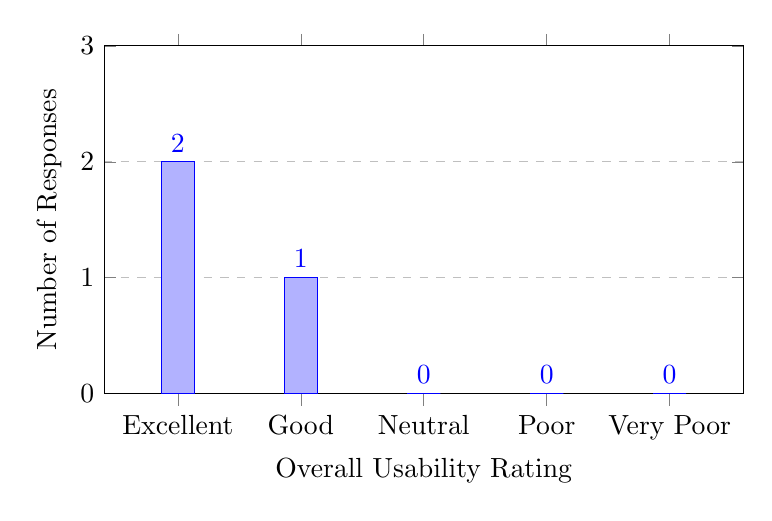
\begin{tikzpicture}
    \begin{axis}[
      ybar,
      bar width=12pt,
      width=0.8\textwidth,
      height=6cm,
      enlarge x limits=0.15,
      ylabel={Number of Responses},
      xlabel={Overall Usability Rating},
      symbolic x coords={Excellent, Good, Neutral, Poor, Very Poor},
      xtick=data,
      nodes near coords,
      ymin=0, ymax=3,
      ymajorgrids=true,
      grid style=dashed,
      ]
      \addplot coordinates {(Excellent,2) (Good,1) (Neutral,0) (Poor,0) (Very Poor,0)};
    \end{axis}
  \end{tikzpicture}
  \caption{Overall Usability Rating}
\end{figure}

\begin{figure}[H]
  \centering
  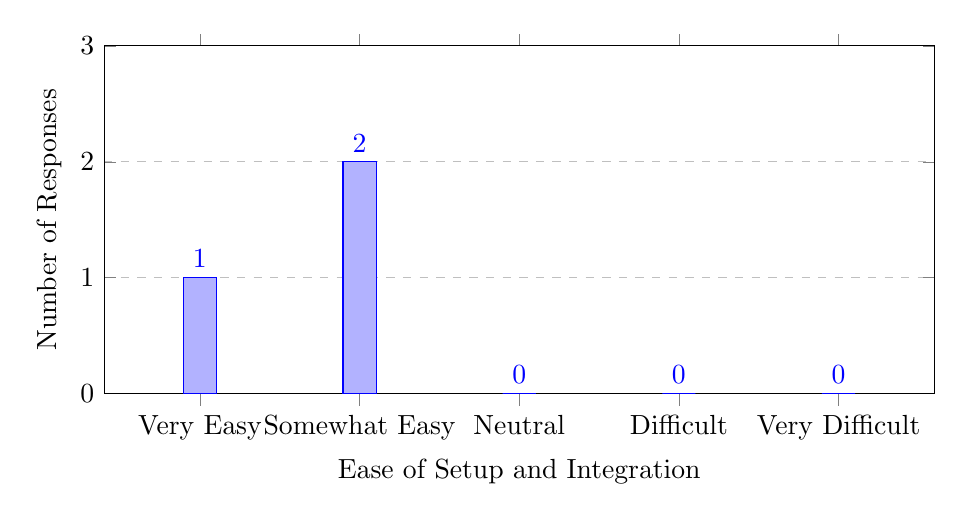
\begin{tikzpicture}
    \begin{axis}[
      ybar,
      bar width=12pt,
      width=1\textwidth,
      height=6cm,
      enlarge x limits=0.15,
      ylabel={Number of Responses},
      xlabel={Ease of Setup and Integration},
      symbolic x coords={Very Easy, Somewhat Easy, Neutral, Difficult, Very Difficult},
      xtick=data,
      nodes near coords,
      ymin=0, ymax=3,
      ymajorgrids=true,
      grid style=dashed,
      ]
      \addplot coordinates {(Very Easy,1) (Somewhat Easy,2) (Neutral,0) (Difficult,0) (Very Difficult,0)};
    \end{axis}
  \end{tikzpicture}
  \caption{Ease of Setup and Integration}
\end{figure}

\begin{figure}[H]
  \centering
  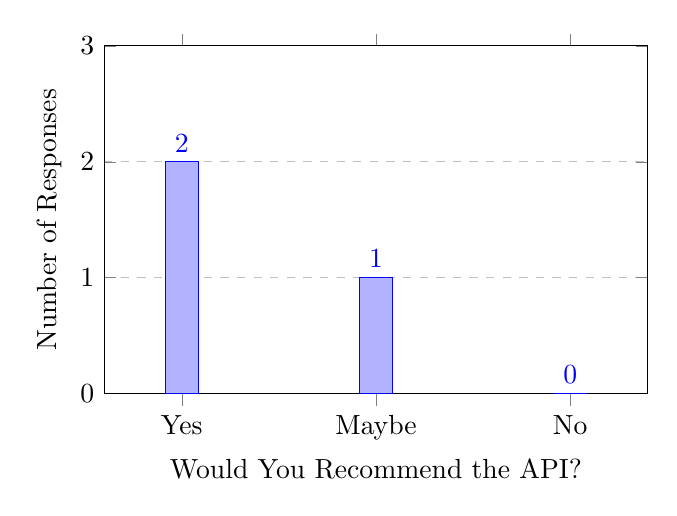
\begin{tikzpicture}
    \begin{axis}[
      ybar,
      bar width=12pt,
      width=0.7\textwidth,
      height=6cm,
      enlarge x limits=0.2,
      ylabel={Number of Responses},
      xlabel={Would You Recommend the API?},
      symbolic x coords={Yes, Maybe, No},
      xtick=data,
      nodes near coords,
      ymin=0, ymax=3,
      ymajorgrids=true,
      grid style=dashed,
      ]
      \addplot coordinates {(Yes,2) (Maybe,1) (No,0)};
    \end{axis}
  \end{tikzpicture}
  \caption{Recommendation Likelihood}
\end{figure}

\subsection{Conclusion}

The solver's API was rated as clear and usable, with minor improvements
suggested for documentation and configurability. All reviewers would recommend
it for use in larger numerical projects, provided additional examples and
higher-level wrappers are included.


\section{Reflection}

The information in this section will be used to evaluate the team members on the
graduate attribute of Reflection.

\input{../Reflection.tex}

% \begin{enumerate}
%   \item What went well while writing this deliverable?
%   \item What pain points did you experience during this deliverable, and how
%     did you resolve them?
%   \item Which parts of this document stemmed from speaking to your client(s) or
%   a proxy (e.g. your peers)? Which ones were not, and why?
%   \item In what ways was the Verification and Validation (VnV) Plan different
%   from the activities that were actually conducted for VnV?  If there were
%   differences, what changes required the modification in the plan?  Why did
%   these changes occur?  Would you be able to anticipate these changes in future
%   projects?  If there weren't any differences, how was your team able to clearly
%   predict a feasible amount of effort and the right tasks needed to build the
%   evidence that demonstrates the required quality?  (It is expected that most
%   teams will have had to deviate from their original VnV Plan.)
% \end{enumerate}

\end{document}
